\documentclass[a4paper,12pt]{report}

% Page layout
\usepackage[left=2.5cm,right=2.5cm,top=2.5cm,bottom=2.5cm]{geometry}

% Font and text
\usepackage[afrikaans,english]{babel}
\usepackage{microtype}
\usepackage{setspace}
\usepackage{lmodern}
\usepackage{siunitx}

\newcommand{\myemph}[1]{{\rmfamily\bfseries#1}}
\sloppy
\onehalfspacing
%\rmfamily  \bfseries
% Headings
\usepackage[raggedright,sf,bf]{titlesec}
\usepackage[margin=\the\parindent,small,bf,sf]{caption}
\titlelabel{\thetitle.\ }
\titleformat{\chapter}[display]{\huge\bfseries\rmfamily }{\chaptertitlename\ \thechapter}{15pt}{\Huge \raggedright}
\titlespacing*{\chapter}{0pt}{0pt}{40pt}  % remove spacing before chapter headings
\makeatletter
\let\originall@chapter\l@chapter
\def\l@chapter#1#2{\originall@chapter{{\rmfamily  #1}}{#2}}
\makeatother
\titleformat*{\section}{\Large\bfseries\rmfamily}
\titleformat*{\subsection}{\large\bfseries\rmfamily}
\titleformat*{\subsubsection}{\bfseries\rmfamily}

%% Alternative headings using small-caps (comment out the top section)
%\usepackage[raggedright,bf]{titlesec}
%\usepackage[margin=\the\parindent,small,bf]{caption}
%\titlelabel{\thetitle.\ }
%\titleformat{\chapter}[display]{\huge\scshape}{\chaptertitlename\ \thechapter}{15pt}{\Huge \raggedright}
%\titlespacing*{\chapter}{0pt}{0pt}{40pt}  % remove spacing before chapter headings

% Table of contents
\let \savenumberline \numberline
\def \numberline#1{\savenumberline{#1.}}

% Figures
\usepackage{graphicx}
\usepackage{pdfpages}
\usepackage{subcaption}
\setlength{\abovecaptionskip}{7.5pt}  % spacing above and below captions
\newcommand*{\WaterMark}[2][0.2\paperwidth]{\AddToShipoutPicture*{\AtTextCenter{\parbox[c]{0pt}{\makebox[0pt][c]{\includegraphics[width=#1]{#2}}}}}}

% Mathematics
\usepackage[cmex10]{amsmath}
\usepackage{amssymb}
\usepackage{cancel}
\DeclareMathOperator*{\argmax}{arg\,max}
\newcommand{\T}{^\top}
\newcommand{\tr}{\textrm{tr}}
\renewcommand{\vec}[1]{\boldsymbol{\mathbf{#1}}}
\newcommand{\defeq}{\triangleq}

% Tables
\usepackage{booktabs}
\usepackage{tabularx}
\usepackage{multirow}
\newcommand{\mytable}{
    \centering
    \small
    \renewcommand{\arraystretch}{1.2}
    }
\renewcommand{\tabularxcolumn}[1]{m{#1}}
\newcolumntype{C}{>{\centering\arraybackslash}X}
\newcolumntype{L}{>{\raggedright\arraybackslash}X}

% Header and footer
\usepackage{fancyhdr}
\pagestyle{fancy}
\fancyhf{}
\renewcommand{\sectionmark}[1]{\markright{\normalsize \thesection.\ #1}}
\fancyhead[C]{\nouppercase{\textit{\rightmark}}}
\fancyhead[RO]{\thepage}
\fancyhead[LE]{\thepage}  % double-sided printing
\fancyfoot{}
\setlength\headheight{14.5pt}
\renewcommand{\headrulewidth}{0pt}
\fancypagestyle{plain}{\fancyhead{}
                       \renewcommand{\headrulewidth}{0pt}
                       \fancyfoot[C]{\thepage}}

% Pseudo-code
\usepackage{algorithm}  % should go before \usepackage{hyperref}

% Table of contents and hyperlinks
\usepackage{hyperref}
\hypersetup{colorlinks=true,linktoc=all,citecolor=black,linkcolor=black, urlcolor=blue}
\usepackage[nottoc]{tocbibind}

% Pseudo-code
\usepackage{algpseudocode}  % should go after \usepackage{hyperref}
\renewcommand{\thealgorithm}{\arabic{chapter}.\arabic{algorithm}} 
\captionsetup[algorithm]{labelfont={bf,sf},font=small,labelsep=colon}

% Bibliography
\usepackage{cite}  % automatically reorder inline citations
\bibliographystyle{IEEEtran}

% Fix titlesec issue
\usepackage{etoolbox}
\makeatletter
\patchcmd{\ttlh@hang}{\parindent\z@}{\parindent\z@\leavevmode}{}{}
\patchcmd{\ttlh@hang}{\noindent}{}{}{}
\makeatother

 \usepackage{booktabs}
 \usepackage{multirow}
% \usepackage[table,xcdraw]{xcolor}
\usepackage{colortbl}

\usepackage{tabularray}

\DeclareSIUnit \amphour {Ah}
\DeclareSIUnit \watthour {Wh}

\begin{document}

% Front matter
\graphicspath{{frontmatter/fig/}}
\pagenumbering{Alph}

\begin{titlepage}
	\begin{center}
		
		
\includegraphics[width=10cm]{SU_corporate_horizontal_with_slogan_RGB}
		
		\vfill
		
		{\rmfamily  \bfseries \huge Development of an air-quality solution for taxis and taxi ranks \par}
		%Air quality measurement and logging in taxi ranks and inside of taxis
%		{\scshape \huge A Critical Analysis of Design Flaws in the Death Star \par}
		
		\vfill
		
		{\large {\Large Willem Cornelis Rossouw} \\ 22823700 \par}
		
		\vfill
		
		\vfill
		
		% Skripsie
		 {\large Report presented in partial fulfilment of the requirements of the module \\ Project (E) 448 for the degree Baccalaureus in Engineering (Electrical and Electronic) in the Faculty of Engineering at Stellenbosch University. \par}

		% Masters (Research)
		%{\large Thesis presented in partial fulfilment of the requirements for the degree of \\ Master of Engineering (Electronic) in the Faculty of Engineering at Stellenbosch University. \par}

		% Masters (Structured)
		% {\large Research assignment presented in partial fulfilment of the requirements for the degree of Master of Engineering (Electronic) \\ in the Faculty of Engineering at Stellenbosch University. \par}

		% PhD
		% {\large Dissertation presented for the degree of Doctor of Philosophy (Electronic Engineering) in the Faculty of Engineering at Stellenbosch University. \par}
		
		\vfill
		
		{\large {Supervisor}: Prof. MJ (Thinus) Booysen } %\\
		% Department of Electrical and Electronic Engineering \par}
		
		\vfill
		
		{\Large May 2023}
	\end{center}
\end{titlepage}

%\graphicspath{{frontmatter/fig/}}
\pagenumbering{Alph}

\begin{titlepage}
	\begin{center}
		
		%\includegraphics[width=10cm]{USlogo-top}
		
		\WaterMark{UScrest-WM}
		
		~\vspace{4.5em}
		
		{\sffamily \bfseries \huge A Critical Analysis of Design Flaws in the Death Star \par}
%		{\scshape \huge A Critical Analysis of Design Flaws in the Death Star \par}		
		
		\vspace{7em}
		
		{\large {\Large  Luke Skywalker} \\ 99652154 \par}
		
		\vspace{8em}
		
		{\large Thesis presented in partial fulfilment of the requirements for the degree of \\ Master of Engineering (Electronic) in the Faculty of Engineering at Stellenbosch University. \par}
		
		\vfill
		
		{\large {Supervisor}: Dr O.\ W.\ Kenobi\\
		Department of Electrical and Electronic Engineering \par}
		
		%\vfill
		\vspace{10em}
		
		{\Large October 2099}
	\end{center}
\end{titlepage}

\pagenumbering{roman}
\chapter*{Acknowledgements}
% \addcontentsline{toc}{chapter}{Acknowledgements}
\makeatletter\@mkboth{}{Acknowledgements}\makeatother

%I would like to thank my dog, Muffin. I also would like to thank the inventor of the incubator; without him/her, I would not be here. Finally, I would like to thank Dr Herman Kamper for this amazing report template.

I would like to thank my supervisor Thinus Booysen for giving me this skripsie topic and for his enthusiasm in his work. I would also like to thank my friend and co-(soon-to-be)-engineer Phillip, for keeping me sane for most of my degree.
%\chapter*{Declaration}
\newpage
\thispagestyle{plain}
\addcontentsline{toc}{chapter}{Declaration}
\makeatletter\@mkboth{}{Declaration}\makeatother

\centerline{
\includegraphics[width=8cm]{US-logo-top}}
\vspace*{-10pt}

\section*{\centering Plagiaatverklaring / \textit{Plagiarism Declaration}}

\vspace*{5pt}

\begin{enumerate}
    \item Plagiaat is die oorneem en gebruik van die idees, materiaal en ander intellektuele eiendom van ander persone asof dit jou eie werk is.\\
    \textit{Plagiarism is the use of ideas, material and other intellectual property of another's work
        and to present is as my own.}
    
    \item Ek erken dat die pleeg van plagiaat 'n strafbare oortreding is aangesien dit 'n vorm van diefstal is.\\
    \textit{I agree that plagiarism is a punishable offence because it constitutes theft.}
    
    \item Ek verstaan ook dat direkte vertalings plagiaat is. \\
    \textit{I also understand that direct translations are plagiarism.}
    
    \item Dienooreenkomstig is alle aanhalings en bydraes vanuit enige bron (ingesluit die internet) volledig verwys (erken). Ek erken dat die woordelikse aanhaal van teks sonder aanhalingstekens (selfs al word die bron volledig erken) plagiaat is. \\
    \textit{Accordingly all quotations and contributions from any source whatsoever (including the internet) have been cited fully. I understand that the reproduction of text without quotation marks (even when the source is cited) is plagiarism}
    
    \item Ek verklaar dat die werk in hierdie skryfstuk vervat, behalwe waar anders aangedui, my eie oorspronklike werk is en dat ek dit nie vantevore in die geheel of gedeeltelik ingehandig het vir bepunting in hierdie module/werkstuk of 'n ander module/werkstuk~nie. \\
    \textit{I declare that the work contained in this assignment, except where otherwise stated, is my original work and that I have not previously (in its entirety or in part) submitted it for grading in this module/assignment or another module/assignment.}
\end{enumerate}

\vfill

\noindent \begin{tabularx}{1.0\linewidth}{|L|L|}
	
    \hline
    
     22823700 &  \raisebox{-21pt}[0pt][0pt]{
\includegraphics[width=2cm, height=1.6cm]{WCsignature.png}}\\

    {Studentenommer / \textit{Student number}}  &  {Handtekening / \textit{Signature}}\\
    \hline
    \vspace{0.2cm}{{W.C. Rossouw}} & \vspace{0.2cm}{ \today }\\
    {Voorletters en van / \textit{Initials and surname}} & {Datum / \textit{Date}}\\
    \hline
\end{tabularx}

\vspace{15pt}

% The old declaration

%I, the undersigned, hereby declare that the work contained in this report is my own original work unless otherwise stated.
%
%% Afrikaans:
%% Hiermee verklaar ek, die ondergetekende, dat die werk in hierdie verslag vervat my eie oorspronklike werk is, tensy anders vermeld.
%
%\vspace{2.5cm}
%
%\begin{table}[h]
%\begin{tabular}{@{}p{2.5cm}p{5cm}}
%    Signature: & \dotfill \\
%    & \multicolumn{1}{c}{Obi-Wan Kenobi} \\
%    ~\vspace{1cm} \\
%    Date: & \dotfill \\
%\end{tabular}
%\end{table}
%
%\vfill
%
%\begin{center}
%    Copyright \textcopyright\ 2099 Stellenbosch University \\
%    All rights reserved
%\end{center}


\chapter*{Abstract}
\addcontentsline{toc}{chapter}{Abstract}
\makeatletter\@mkboth{}{Abstract}\makeatother

\subsubsection*{English}

The English abstract.

\selectlanguage{afrikaans}

\subsubsection*{Afrikaans}

Die Afrikaanse uittreksel.

\selectlanguage{english}

%change depth of table of contents

\setcounter{tocdepth}{3}
\setcounter{secnumdepth}{3}
\tableofcontents
\listoffigures
\listoftables
\chapter*{Nomenclature\markboth{}{Nomenclature}}
\addcontentsline{toc}{chapter}{Nomenclature}

% \vspace*{-3mm}
%\subsubsection*{Variables and functions}
%
%\begingroup
%\renewcommand{\arraystretch}{1.2}
%\renewcommand{\tabularxcolumn}[1]{p{#1}}
%\begin{tabularx}{\textwidth}{@{}p{2.5cm}L}
%    $p(x)$ & Probability density function with respect to variable $x$.\\
%    $P(A)$ & Probability of event $A$ occurring.\\
%    $\varepsilon$ & The Bayes error. \\
%    $\varepsilon_u$ & The Bhattacharyya bound. \\
%    $B$ & The Bhattacharyya distance. \\
%    $s$ & An HMM state.  A subscript is used to refer to a particular state, e.g.\ $s_i$ refers to the $i^{\text{th}}$ state of an HMM. \\
%    $\mathbf{S}$ & A set of HMM states. \\
%    $\mathbf{F}$ & A set of frames. \\
%    $\mathbf{o}_f$ & Observation (feature) vector associated with frame $f$. \\
%    $\gamma_s(\mathbf{o}_f)$ & A posteriori probability of the observation vector $\mathbf{o}_f$ being generated by HMM state $s$. \\
%    $\mu$ & Statistical mean vector. \\
%    $\Sigma$ & Statistical covariance matrix. \\
%    $L(\mathbf{S})$ & Log likelihood of the set of HMM states $\mathbf{S}$ generating the training set observation vectors assigned to the states in that set. \\
%    $\mathcal{N}(\mathbf{x} | \mu, \Sigma)$ & Multivariate Gaussian PDF with mean $\mu$ and covariance matrix $\Sigma$.\\
%    $a_{ij}$ & The probability of a transition from HMM state $s_i$ to state $s_j$. \\
%    $N$ & Total number of frames or number of tokens, depending on the context. \\
%    $D$ & Number of deletion errors. \\
%    $I$ & Number of insertion errors. \\
%    $S$ & Number of substitution errors. \\
%\end{tabularx}
%\endgroup


%\newpage
\subsubsection*{Acronyms and abbreviations}

\begingroup
\renewcommand{\arraystretch}{1.2}
\begin{tabular}{@{}p{2.5cm} l}

	PM		& Particulate Matter\\
	VOC		& Volatile Organic Compounds\\
	UART	& Universal Asynchronous Receiver / Transmitter\\
	i2c		& Inter-Integrated Circuit\\
	UFP		& Ultrafine Particle\\
	LPG		& Liquefied Petroleum Gas\\
	CNG 	& Compressed Natural Gas\\
	PPM		& Parts Per Million\\
	PPB		& Parts Per Billion\\
	NDIR	& Nondispersive Infrared\\
	PID		& Photoionization Detector\\
	FID		& Flame Ionization Detector\\
	MOS		& Oxide Semiconductor Sensor\\
	UV		& Ultraviolet\\
	AQI		& Air Quality Index\\
	IO		& Inputs and Outputs\\
	HAT		& Hardware Attached on Top\\
	
\end{tabular}
\endgroup

\newpage
\pagenumbering{arabic}

% Contents
\graphicspath{{introduction/fig/}}

\chapter{Introduction}
\label{chap:introduction}

\section{Background}
In South Africa, millions of commuters use taxis frequently and depend on them for all of their mobility needs \cite{depttransport2023}.\\
The South African government has recognised the impact of taxi emissions on air quality and has taken steps to address the issue. In 2006, the government gazetted regulations that required taxi operators to convert their vehicles to run on cleaner fuels, such as liquefied petroleum gas (LPG), compressed natural gas (CNG), or diesel with lower sulphur content\cite{2007Comparison}. 

\begin{figure}[!htb]
	\minipage{0.32\textwidth}%
	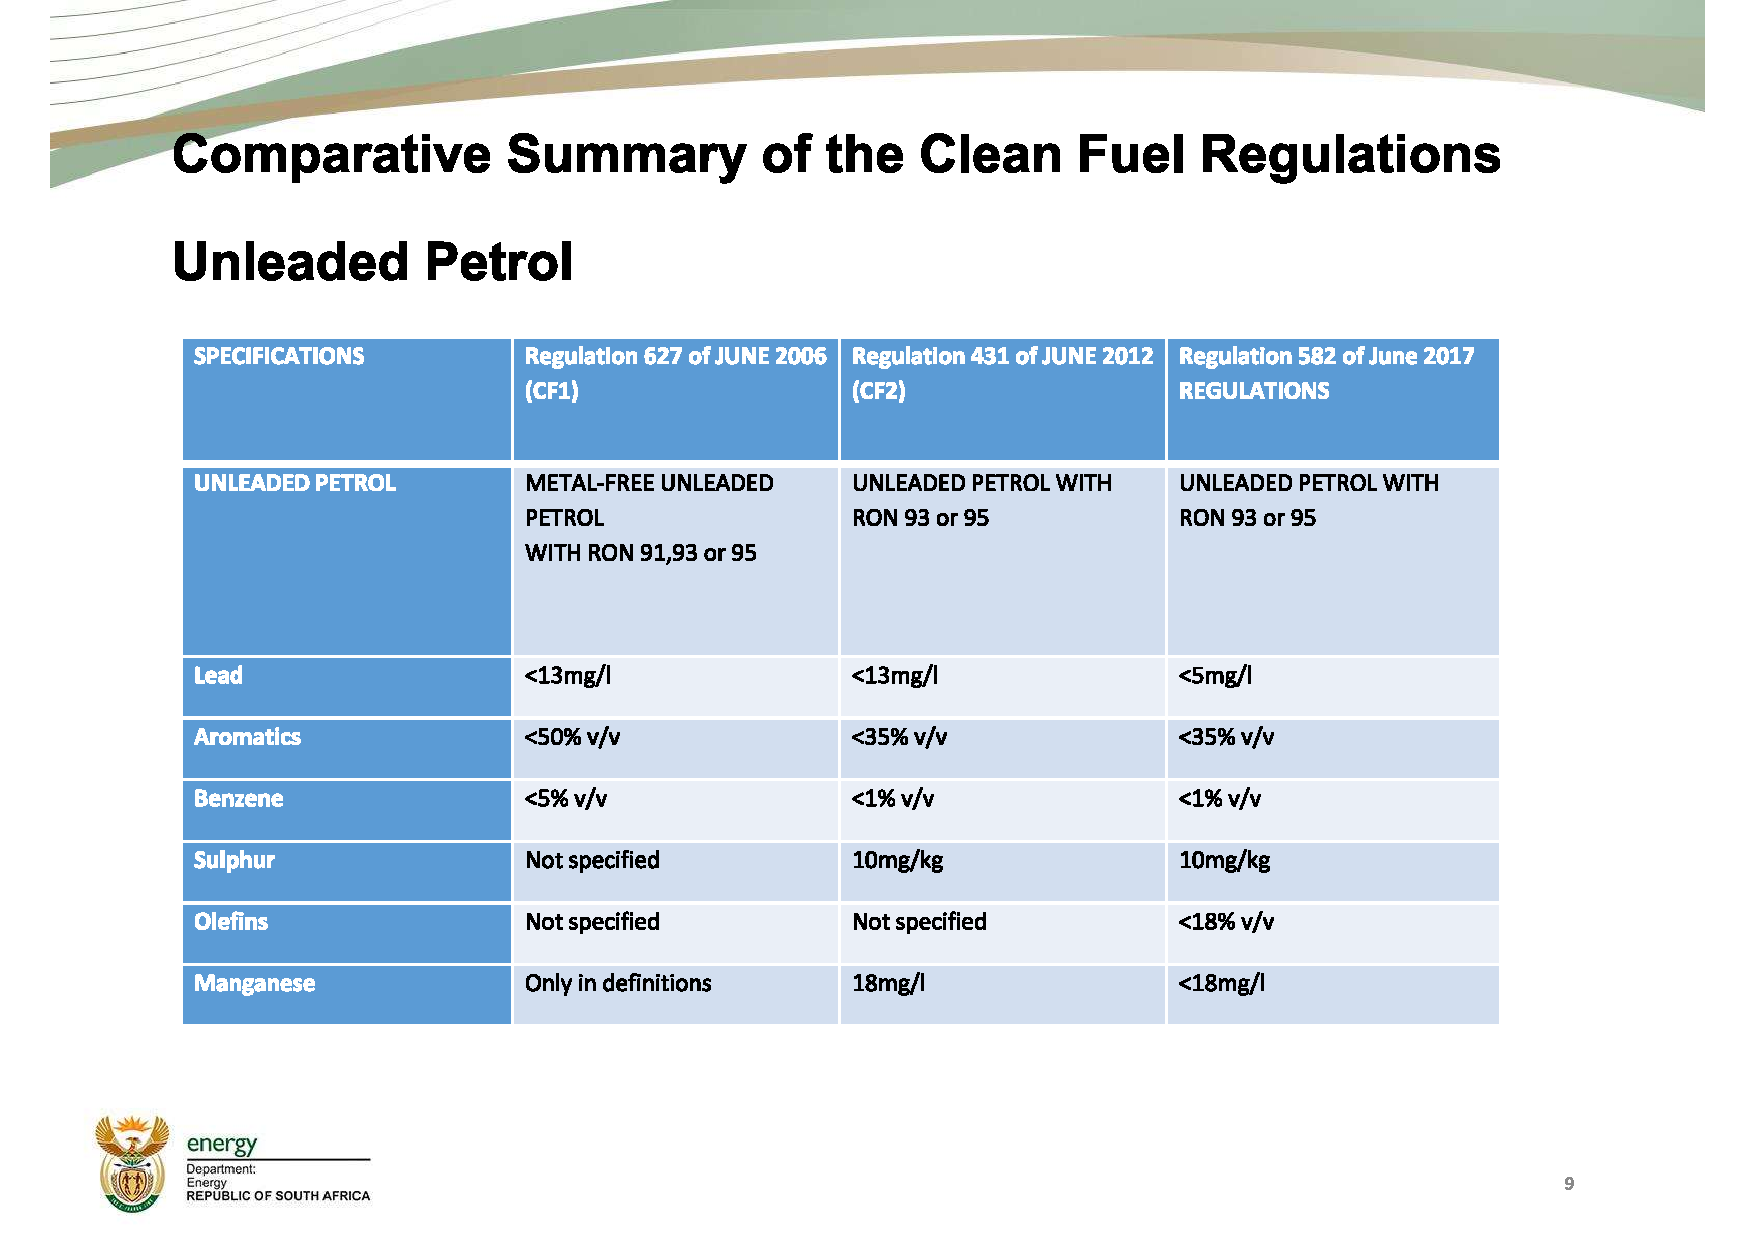
\includegraphics[width=\linewidth]{introduction/fig/page1Comp.pdf}
	\caption{Unleaded\cite{2007Comparison}}\label{fig:fig1}
	\endminipage\hfill
	\minipage{0.32\textwidth}%
	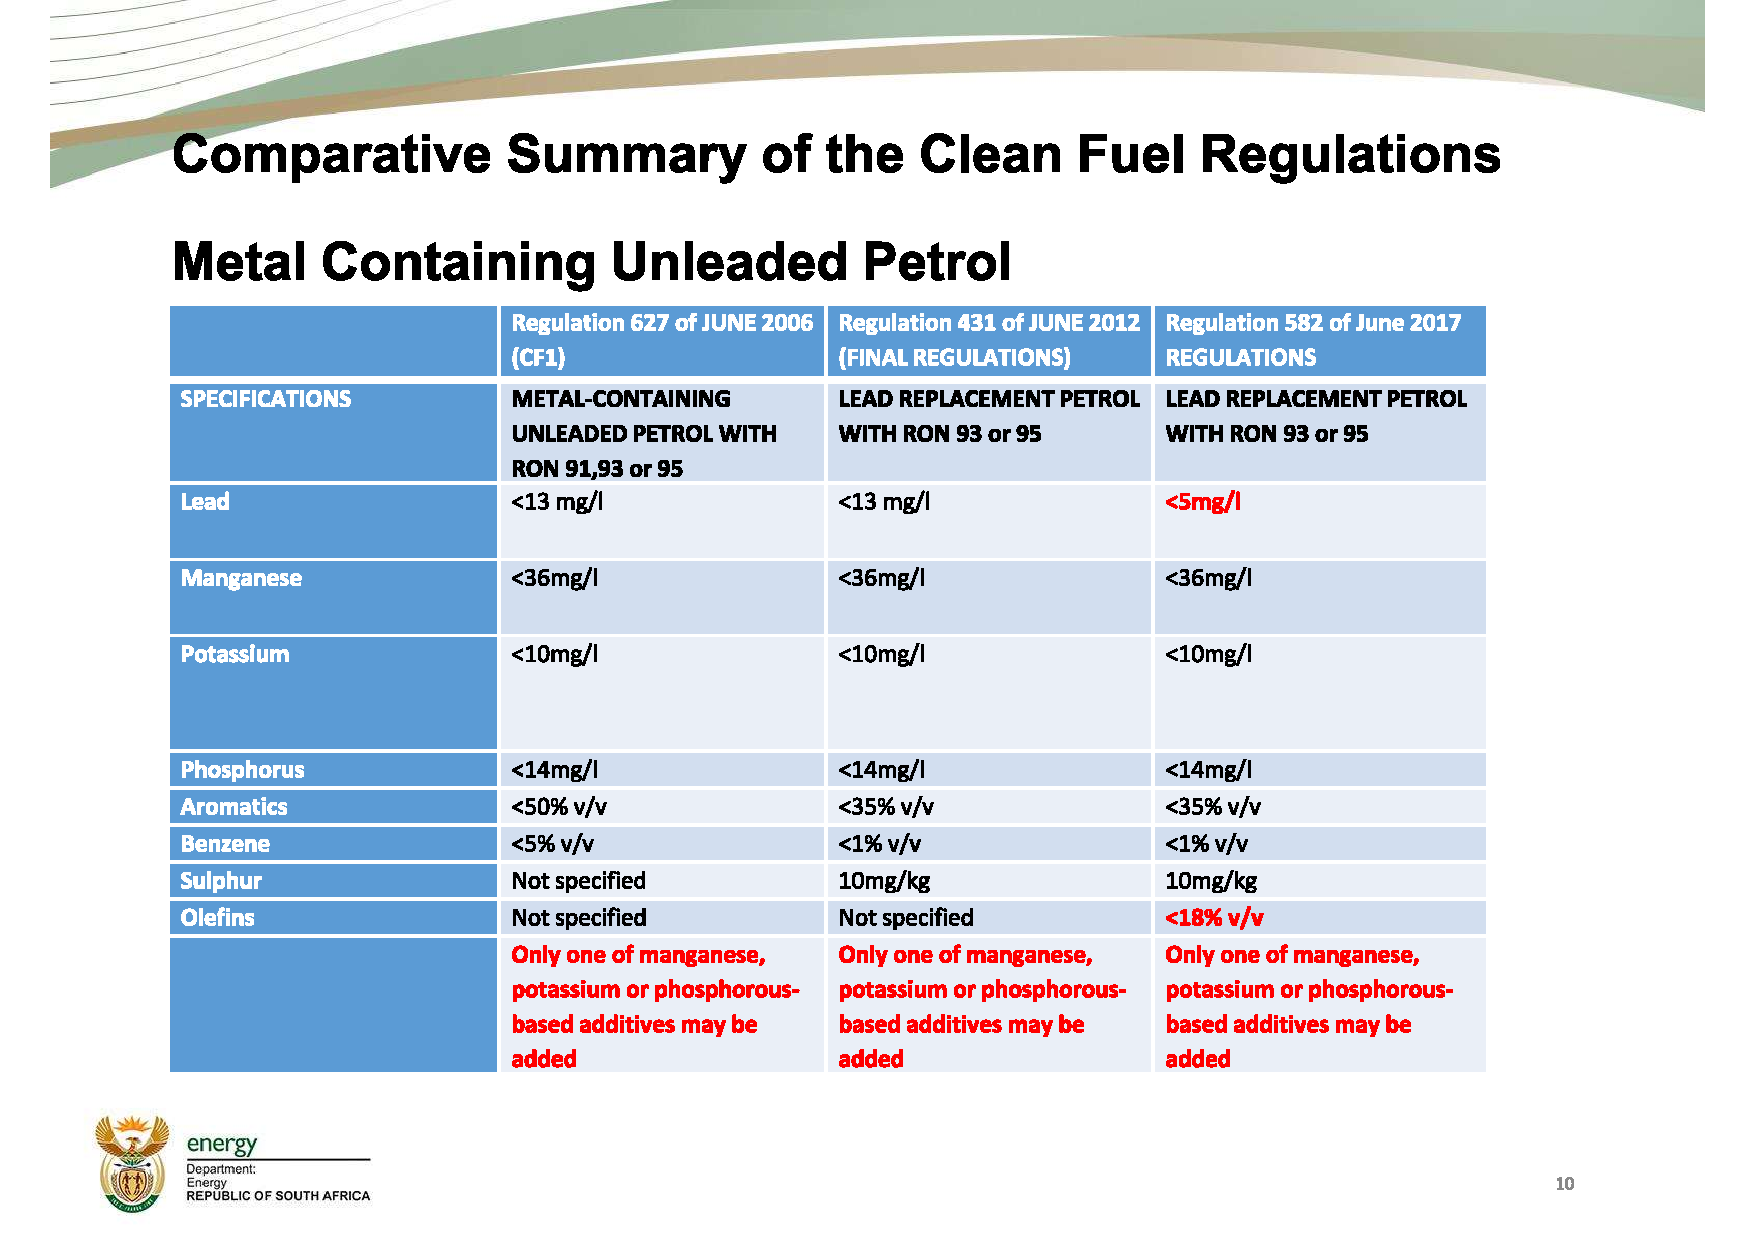
\includegraphics[width=\linewidth]{introduction/fig/page2Comp.pdf}
	\caption{Metal+ Unleaded\cite{2007Comparison}}\label{fig:fig2}
	\endminipage\hfill
	\minipage{0.32\textwidth}%
	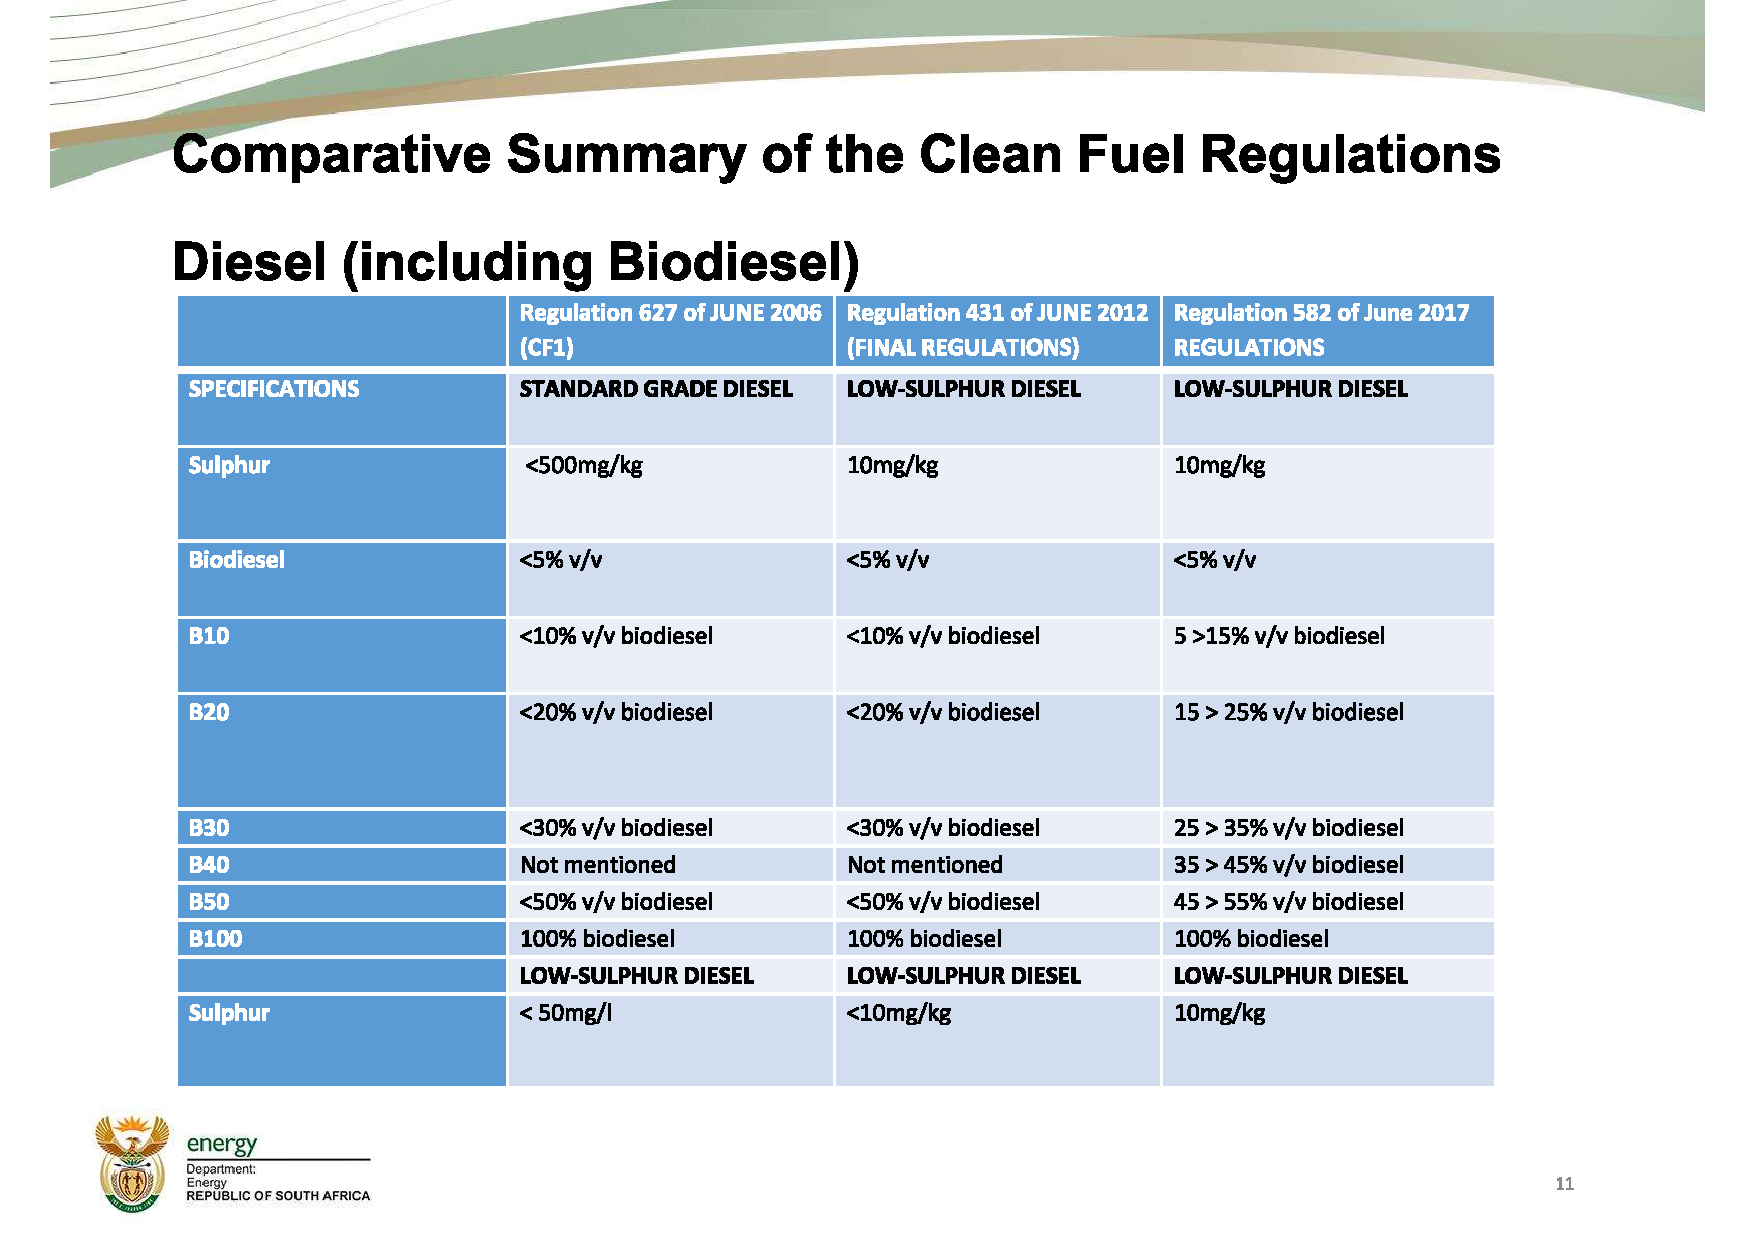
\includegraphics[width=\linewidth]{introduction/fig/page3Comp.pdf}
	\caption{Diesel\cite{2007Comparison}}\label{fig:fig3}
	\endminipage
	%\text{Charts provided by \cite{2007Comparison}}
\end{figure}

\noindent
As seen in Figures \ref{fig:fig1}, \ref{fig:fig2} and \ref{fig:fig3}, South Africa's regulations on cleaner fuels are updated every five to six years. Cleaner fuels produce less greenhouse emissions. The implementation of these regulations has been slow and often poorly regulated \cite{newcleanfuelstandards}, resulting in continued poor air quality in many areas.

\noindent
The main sources of air pollution in South Africa are industrial activities, power generation, vehicle emissions, biomass burning, and domestic fuel use \cite{Bylaws2023}. Among these sources, vehicle emissions are particularly relevant for taxi commuters, who are exposed to high levels of pollutants such as particulate matter (PM), nitrogen oxides (NOx), carbon monoxide (CO), and volatile organic compounds (VOCs) \cite{Venter2018}. These pollutants can have adverse effects on respiratory, cardiovascular, neurological, and immune systems, as well as increase the risk of cancer and premature death \cite{WHO2016}.

%Instead of using expensive and inconvenient formal public transportation like buses and trains, they offer an accessible and affordable substitute.

%{\color{red} \huge Need to rewrite}
\section{Problem Statement}
Despite the popularity and importance of taxis in South Africa, there is a lack of research on the air quality inside these vehicles and at taxi ranks. 
Air quality is a crucial factor for human health and well-being, especially for commuters who spend long hours in taxis exposed to various pollutants.
Moreover, taxi emissions contribute to the overall air pollution in crowded spaces (in this case taxi ranks), which affects the environment and the quality of life of the passers by. The closest studies are concerning single cab taxis\cite{insidetaxismall}, road based pollution\cite{taxiNetwork} and general pollution\cite{Environmentalimpact}.
There is a need for a study on the air quality in taxis and taxi ranks and its impacts on human health and the environment, this report aims to provide a means to that end.

\section{Objectives}
The objective of the study are as follows:
\begin{itemize}
	\item To design a device to measure the levels of:
		\begin{itemize}
			\item CO2
			\item VOC
			\item NOx
			\item Particulate Matter
		\end{itemize}
	%	 CO2, VOC, particulate matter and NOx
 both inside taxis and in taxi ranks.
%	\item Identify the primary sources of air pollution in taxi ranks and within taxis and evaluate the impact of environmental factors, such as traffic congestion and weather conditions(optional- time limited).
	\item To investigate the potential health risks associated with exposure to air pollution in taxi ranks and within taxis, particularly for passengers, drivers and potential third parties.
%	\item To evaluate the effectiveness of current measures in place to reduce air pollution from taxis, such as emission standards and regulations.
	\item Develop hardware that measures the above-mentioned.
	\item Develop software/firmware that integrates the hardware.
%	\item Propose potential strategies to mitigate the impact of  from taxis on public health and the environment such as implementing new technologies.
\end{itemize}


%\section{Summary of Work}??


\section{Scope}
The scope of the project encompasses only the following:

\begin{itemize}
	\item Design of base station and satellite module
	\item Design of communication network for satellite module and base station as well as data storage and backup
	%\item Deployment of sensor and network
%	\item Analysis of data gathered
	\item Hardware development
	\item Software development
	\item Test of Hardware and Software elements
\end{itemize}

\section{Report Overview}%Roadmap


{\color{red}  \LARGE NEED TO DO THIS}








%This is some section with two table in it: Table~\ref{tbl:exemplars} and Table~\ref{tbl:abx_speaker}.

%	\begin{table}[!h]
%	    \mytable
%	    \caption{Performance of the unconstrained segmental Bayesian model on TIDigits1 over iterations in which the reference set is refined.}
%	    \begin{tabularx}{\linewidth}{@{}lCCCCC@{}}
%	        \toprule
%	        Metric     & 1 & 2 & 3 & 4 & 5 \\
%	        \midrule
%	        WER (\%)                        & $35.4$ & $23.5$ & $21.5$ & $21.2$ & $22.9$ \\
%	        Average cluster purity (\%)       & $86.5$ & $89.7$ & $89.2$ & $88.5$ & $86.6$ \\
%	        Word boundary $F$-score (\%)         & $70.6$ & $72.2$ & $71.8$ & $70.9$ & $69.4$ \\
%	        Clusters covering 90\% of data   & 20             & 13 & 13 & 13 & 13 \\
%	        \bottomrule
%	    \end{tabularx}
%	    \label{tbl:exemplars}
%	\end{table}


%\begin{table}[!h]
%    \renewcommand{\arraystretch}{1.1}
%    \centering
%    \caption{A table with an example of using multiple columns.}
%    \begin{tabularx}{0.65\linewidth}{@{}lCCr@{}}
%        \toprule
 %       & \multicolumn{2}{c}{Accuracy (\%)} \\
%        \cmidrule(lr){2-3}
%        Model    & Intermediate & Output & Bitrate\\
%        \midrule
%        Baseline & 27.5         & 26.4   & 116 \\
%        VQ-VAE   & 26.0         & 22.1   & 190 \\
%        CatVAE   & 28.7         & 24.3   & 215 \\
 %    \end{tabularx}
%    \label{tbl:abx_speaker}
%\end{table}

%\newpage

%This is a new page, showing what the page headings looks like, and showing how to refer to a figure like Figure~\ref{fig:cae_siamese}.

%\begin{figure}[!t]
%    \centering
%%     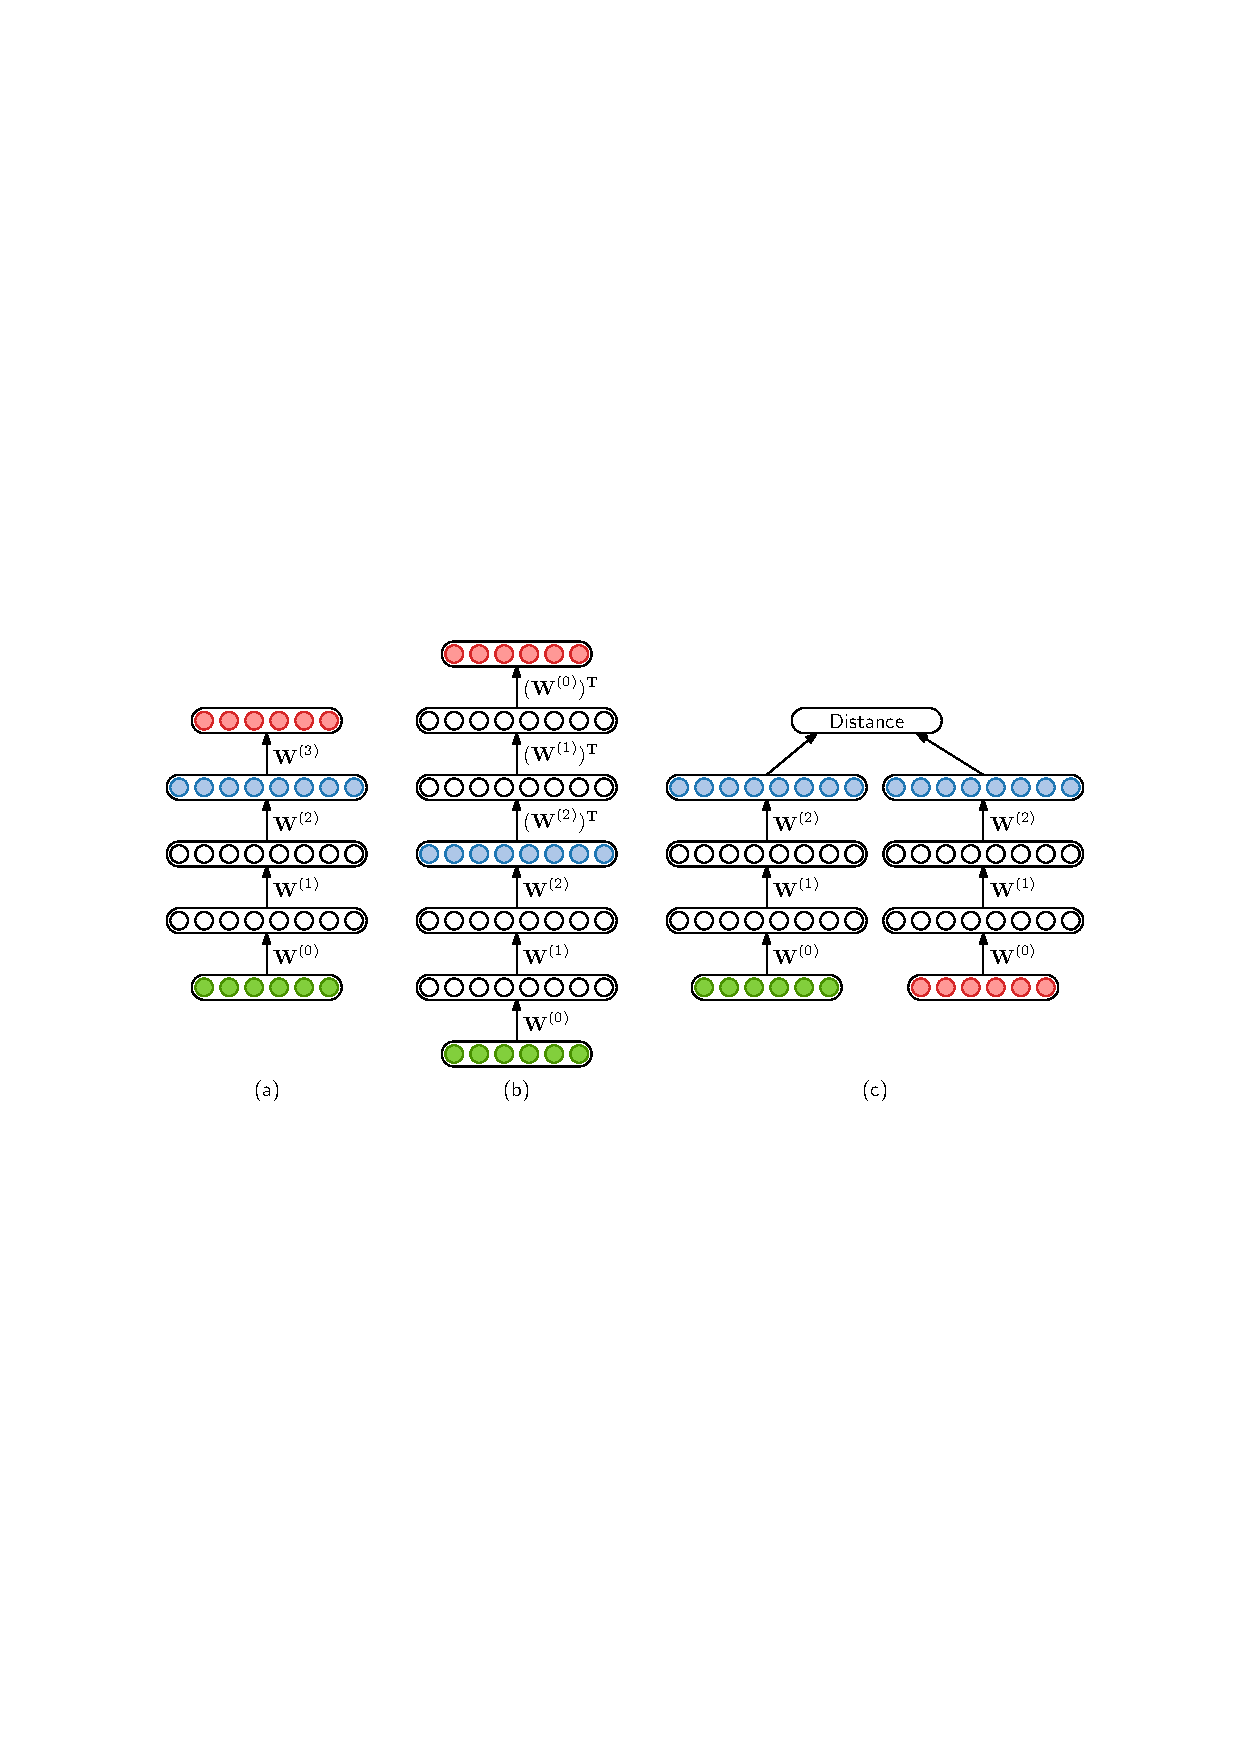
\includegraphics[width=\linewidth]{cae_siamese}
%    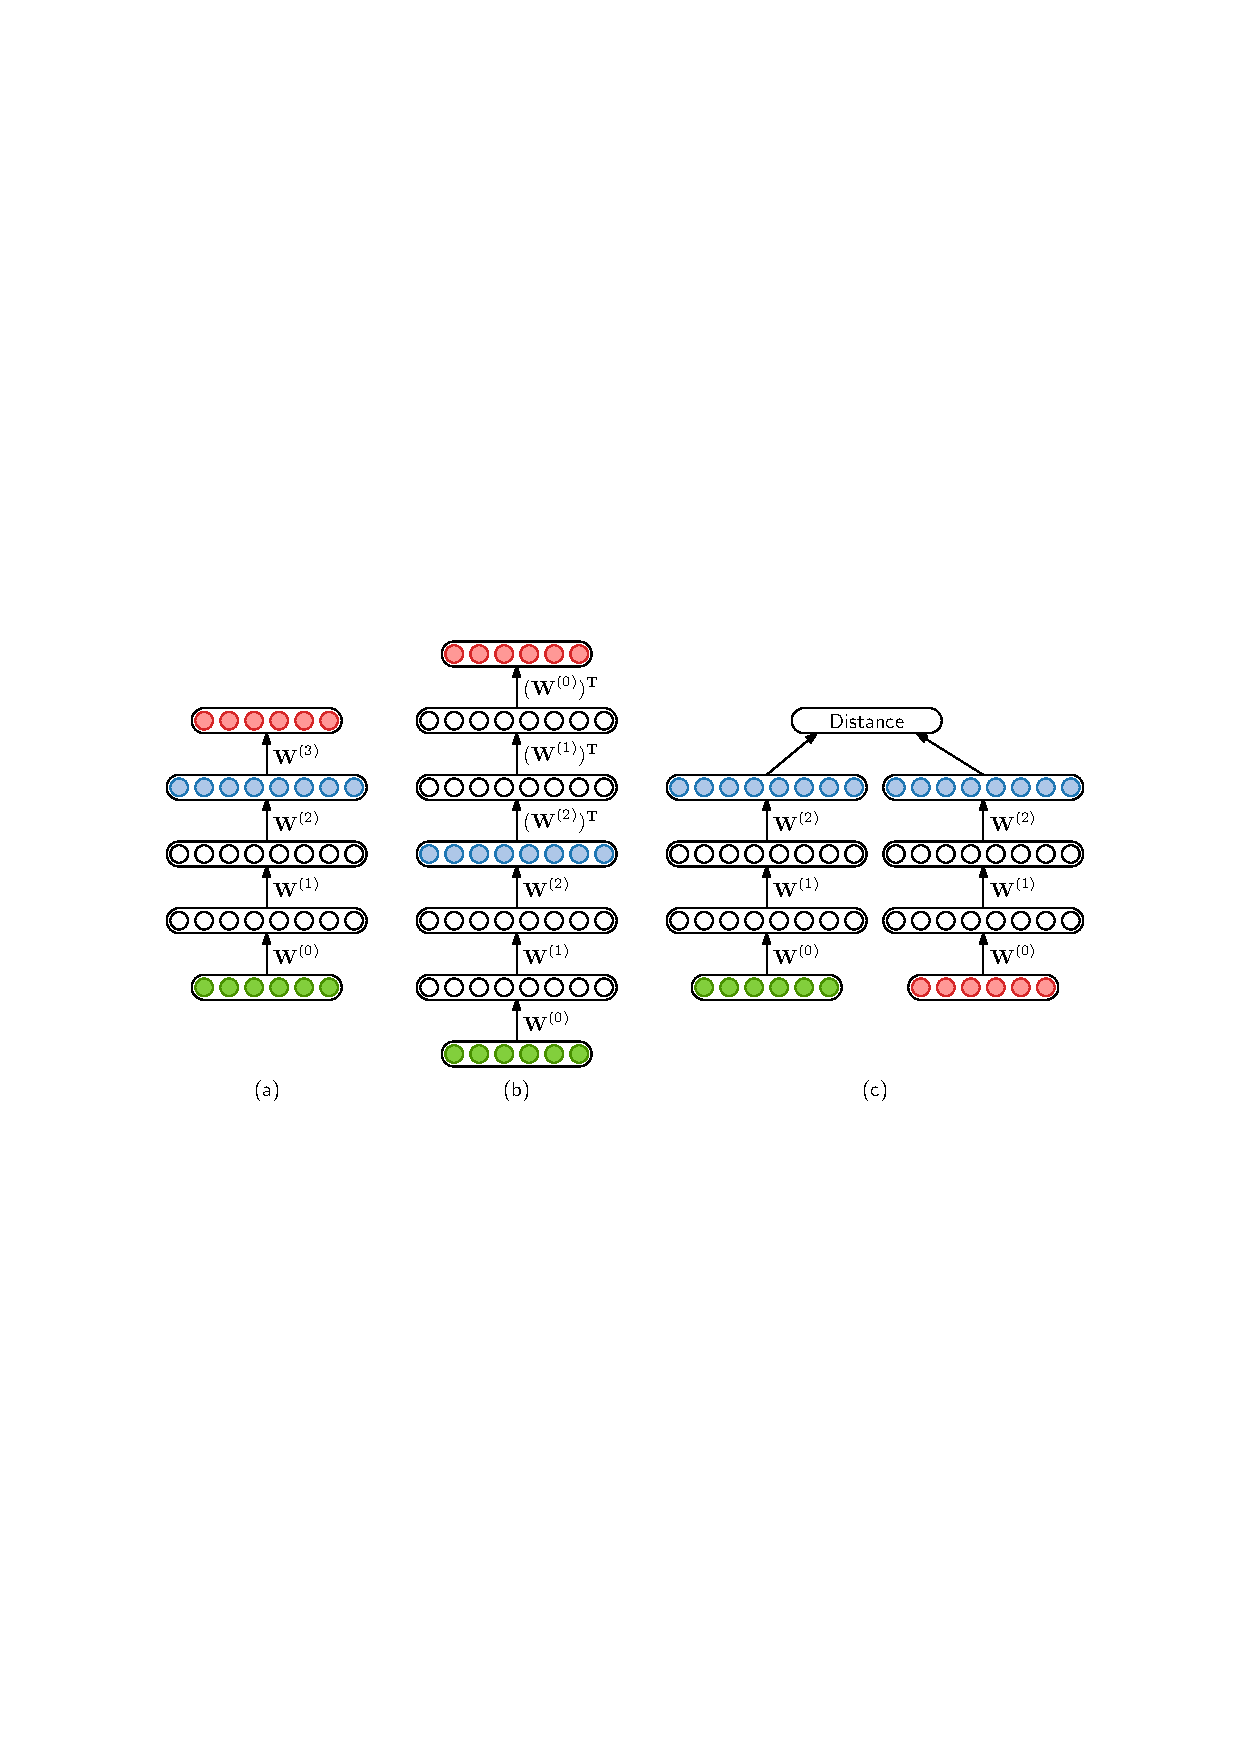
\includegraphics[width=0.918\linewidth]{cae_siamese}
%    \caption[I am the short caption that appears in the list of figures, without references.]{
%    (a) The cAE as used in this chapter. The encoding layer (blue) is chosen based on performance on a development set.
%    (b) The cAE with symmetrical tied weights. The encoding from the middle layer (blue) is always used.
%    (c) The siamese DNN. The cosine distance between aligned frames (green and red) is either minimized or maximized depending on whether the frames belong to the same (discovered) word or not.
%    A cAE can be seen as a type of DNN.
%    }
%    \label{fig:cae_siamese}
%\end{figure}

%
%The following is an example of an equation:
%\begin{equation}
%P(\vec{z} | \vec{\alpha}) = \int_{\vec{\pi}} P(\vec{z} | \vec{\pi}) \, p(\vec{\pi} | \vec{\alpha}) \, \textrm{d} \vec{\pi}
%= \int_{\vec{\pi}} \prod_{k = 1}^K \pi_k^{N_k} \frac{1}{B(\vec{\alpha})} \prod_{k = 1}^K \pi_k^{\alpha_k - 1} \, \textrm{d} \vec{\pi}
%\label{eq:example_equation}
%\end{equation}
%which you can subsequently refer to as~\eqref{eq:example_equation} or Equation~\ref{eq:example_equation}.
%But make sure to consistently use the one or the other (and not mix the two ways of referring to equations).
\chapter{Literature Study}
\chapter{System Design}
%System design with system diagram



\begin{figure}[!htb]
	\centering
	\includegraphics[width=\textwidth]{body/fig/Fulldrawio}
	\caption{Hardware and Interface Overview \\(Base station on the left and Satellite station on the right) }
	\label{fig:fulldrawio}
\end{figure}


\section{Microcontroller}

\section{ESPNow/WiFi}

\section{Sensors}
\subsection{$\mathbf{CO_2}$}
% why was it chosen
\subsection{PM, $\mathbf{NO_x}$, VOC}

\section{Metrics}
%Does the sensor actually work...
%Does it work as wanted
%Experimental setup
\chapter{Detailed System Design}
\vspace{-2em}
\section{Hardware}


This system consists of multiple interconnecting components that will be discussed in detail in this section, namely:
\begin{itemize}
	\item ESP32-S2
	\item Sensiron Sen55
	\item Senseair K30
	\item SD-card adapter
	\item ATGM336H GPS module	
\end{itemize} 




\subsection{ESP32-S2}

\begin{figure}[!htb]
	\centering
	\includegraphics[width=0.4\linewidth]{body/fig/s2_mini}
	\caption{ESP32-S2 mini}
	\label{fig:s2mini}
\end{figure}


\noindent
The module used is the ESP32-S2 mini by WEMOS/Lolin. This module features thirty seven digital pins, three SPI interfaces with two of them fully available, two i2c buses, dual hardware UARTs, a built-in WiFi radio with antenna on board. The board runs on 3.3v power, but has an onboard voltage regulator that works on 5V. Although the board supports multiple i2c devices, it was chosen to connect both devices to one bus since they have different addresses. This also alleviates some space in memory by not having another initialisation of the i2c library instance. The board features an ultra low power co-processor capable of waking up from i2c interrupts, this could be used if deploying for longer durations. The main processor is an {Xtensa\textregistered}  32 bit Single Core Microprocessor that operates at up to 240MHz. Should this device be deployed with only internet capability in a data sensitive environment it also features cryptographic hardware accelerators. The board features native support for USB and does not need a serial bus bridge, making debugging much easier. It is also rated for extreme conditions, capable of working at up to 120 degrees Celsius\cite{wemos2021s2mini}.


\subsection{Sensirion SEN55}
\begin{figure}[!htb]
	\centering
	\includegraphics[width=0.7\linewidth]{body/fig/SEN5x}
	\caption{Sensirion SEN55}
	\label{fig:sen5x}
\end{figure}
\noindent
This sensor provides Particulate Matter, Relative Humidity, Temperature, VOC Index and NOx Index outputs.
It is produced by Sensirion and uses a ACES 51452-006H0H0-001 connector interface to connect. It communicates using the i2c bus and has a library available to use to read its values, however, the NOx and VOC outputs are in the format of an index and the raw values are available but the conversion algorithm is proprietary, the index is thus used. The board uses 5v power as its VCC but communicates over i2c at 3.3V common voltage. The 5V is provided straight from the power bank in this use case.
For the readings from the sensor, the particulate matter, relative humidity and temperature values are available immediately, with the VOC value following shortly behind. For the NOx and VOC values to be reliable, the sensor needs to be in operation for 1 hour for VOC and 6 hours for NOx. For extended use, as would be the case in the taxi rank, the sensor has a learning function on the VOC and NOx index, which is set by default as 12 hours. From this the sensor will estimate the mean gain for the previous 12 hours. The device also features a self cleaning mode, this runs once a week.


\subsection{Senseair K30}
\begin{figure}[!htb]
	\centering
	\includegraphics[width=0.6\linewidth]{body/fig/k30fr}
	\caption{Senseair K30 FR}
	\label{fig:k30fr}
\end{figure}
The Senseair K30 FR module is an NDIR $ CO_2 $ sensor with 5000 ppm sensing range and an accuracy of 3\%. It has a rate of measurement of 2 Hz and a response time of 2 seconds, but since we are not using a gas tube, the diffusion time is 20 seconds which should be appropriate for the application. The sensor has a few ways to interface with the microcontroller, it features two analog outputs of 0 to 5V and 0 to 10V respectively representing 0 to 5000 ppm. It also features UART utilizing the MODBUS protocol as well as i2c communication. The sensor runs on 5 to 14V for power and has a dedicated input for the communications voltage, allowing the microcontroller to communicate at 3.3 or 5V depending on the model. The sensor communication is done using i2c and there is a detailed document by Sensair describing the protocol. The module also features the ability to change its address, this persists through power down, this negates the issue of having two sensors with the same address conflicting in the case of default addresses. 
\begin{figure}[!htb]
	\centering
	\includegraphics[width=0.6\linewidth]{body/fig/i3ck30}
	\caption[i2c for K30]{The i2c lines SDA and SDL are defined on the factory connector as well as the G+ and G0 representing VCC 5V in this case and ground along with DVCC representing the 3.3V communications voltage.}
	\label{fig:i3ck30}
\end{figure}
\pagebreak
\subsection{ATGM336H GPS module}

\begin{figure}[!htb]
	\minipage{0.4\textwidth}%
	\includegraphics[width=\textwidth]{body/fig/NEO_M8_N_MOD_001}
	\caption{ATGM336H}
	\label{fig:neom8nmod001}
	\endminipage\hfill
	\minipage{0.4\textwidth}%
	\includegraphics[width=\textwidth]{body/fig/GPSant.png}
	\caption[GPS Antenna]{GPS Antenna}
	\label{fig:gps-1ant}
	\endminipage\hfill
\end{figure}
\noindent
The GPS module chosen for the satellite station is the \href{https://www.robotics.org.za/NEO-M8N-MOD}{ATGM336H} shown in Figure~\ref{fig:neom8nmod001}, it is a small module, measuring in at only 13.1 by 15.7mm. It operates at $3.3 \si{\volt}$ and consumes only $25 \si{\milli\ampere}$ when acquiring its position for the first time, and  $20 \si{\milli\ampere}$ while tracking. It has an accuracy of 2.5 meters and an update rate of 10 Hz although 1 Hz is standard. The time to first fix for this module, referring to the time it needs to acquire an accurate location without the help of cell towers, is 26 seconds, this is also referred to as a cold start. Once it has the initial fix, it refreshes every second, and also supplies a PPS or pulse per second as a heartbeat. The module uses UART or Serial to communicate at a default Baud Rate of 9600bps. The standard it uses to communicate is NMEA0183, this will be further discussed in the software design. The module also includes a ceramic antenna, but another flat Molex Flexible GPS Antenna was used to allow the unit to not be as susceptible to bumps and outside interference.
The \href{https://www.robotics.org.za/GPS-15246?search=antenna}{GPS Antenna} shown in Figure~\ref{fig:gps-1ant} is the antenna used in the design, it also features greater than 74\% efficiency and is only 0.1 mm thick with an adhesive backing making it extremely easy to mount.

\pagebreak
\subsection{SD-card adapter}
\begin{figure}[!htb]
	\centering
	\includegraphics[width=0.5\linewidth]{body/fig/MICRO-SD-PTL-005}
	\caption{SD card adapter}
	\label{fig:micro-sd-ptl-005}
\end{figure}

\noindent
The micro SD card adapter/module chosen is a simplistic connector, merely relaying the SPI connectors from the micro SD card to the SPI pins on the microcontroller. It runs on 3.3V and features low quiescent current when not used. The SD card itself is limited by the SPI and library limitations, limiting its size to $ 32 \si{\giga\byte} $ The SD card used can be variable by design, and the limiting factor will ultimately be the size of the files on the SD card, as they have to be transferred, The 24 hour data used approximately $ 1 \si{\mega\byte} $ of storage with 8640 data points. This means the card itself will likely not be the bottleneck. 16 $ 16 \si{\giga\byte} $ card were used for this project simply because they were readily available and rather affordable.




%The ESP32-S2 is capable of multiple STA and AP modes, including simultaneous broadcasting over ESP-NOW and WiFi. This is needed to be able to have the 2 ESP boards communicate and the base station be able to send the data to a database.
%\subsection{SD - interface}
%The SD card interface was done using SPI. The module was hard soldered to a micro SD to SD card adapter. These pins were then soldered to the ESP32's SPI and 3.3V pins.
%The FS, SD and SPI libraries from Espresiff were used to interface with the already formatted micro SD card.



%
%\subsection{Sensors}
%\subsubsection{$\mathrm{CO_2}$}
%{\color{red} \huge Insert docs you made while working with them}
%
%% why was it chosen
%
%
%\subsubsection{PM, $\mathrm{NO_x}$, VOC, Temperature, Humidity}
%\noindent
%The main ESP referenced as the Base station, will be connected periodically to the internet to send the data it collects to the database of choice. 


\pagebreak
\subsection{Software/Firmware implementation}
\subsubsection{Overview}
%{\color{red} \huge Insert flowchart}

\begin{figure}[!htb]
	\centering
	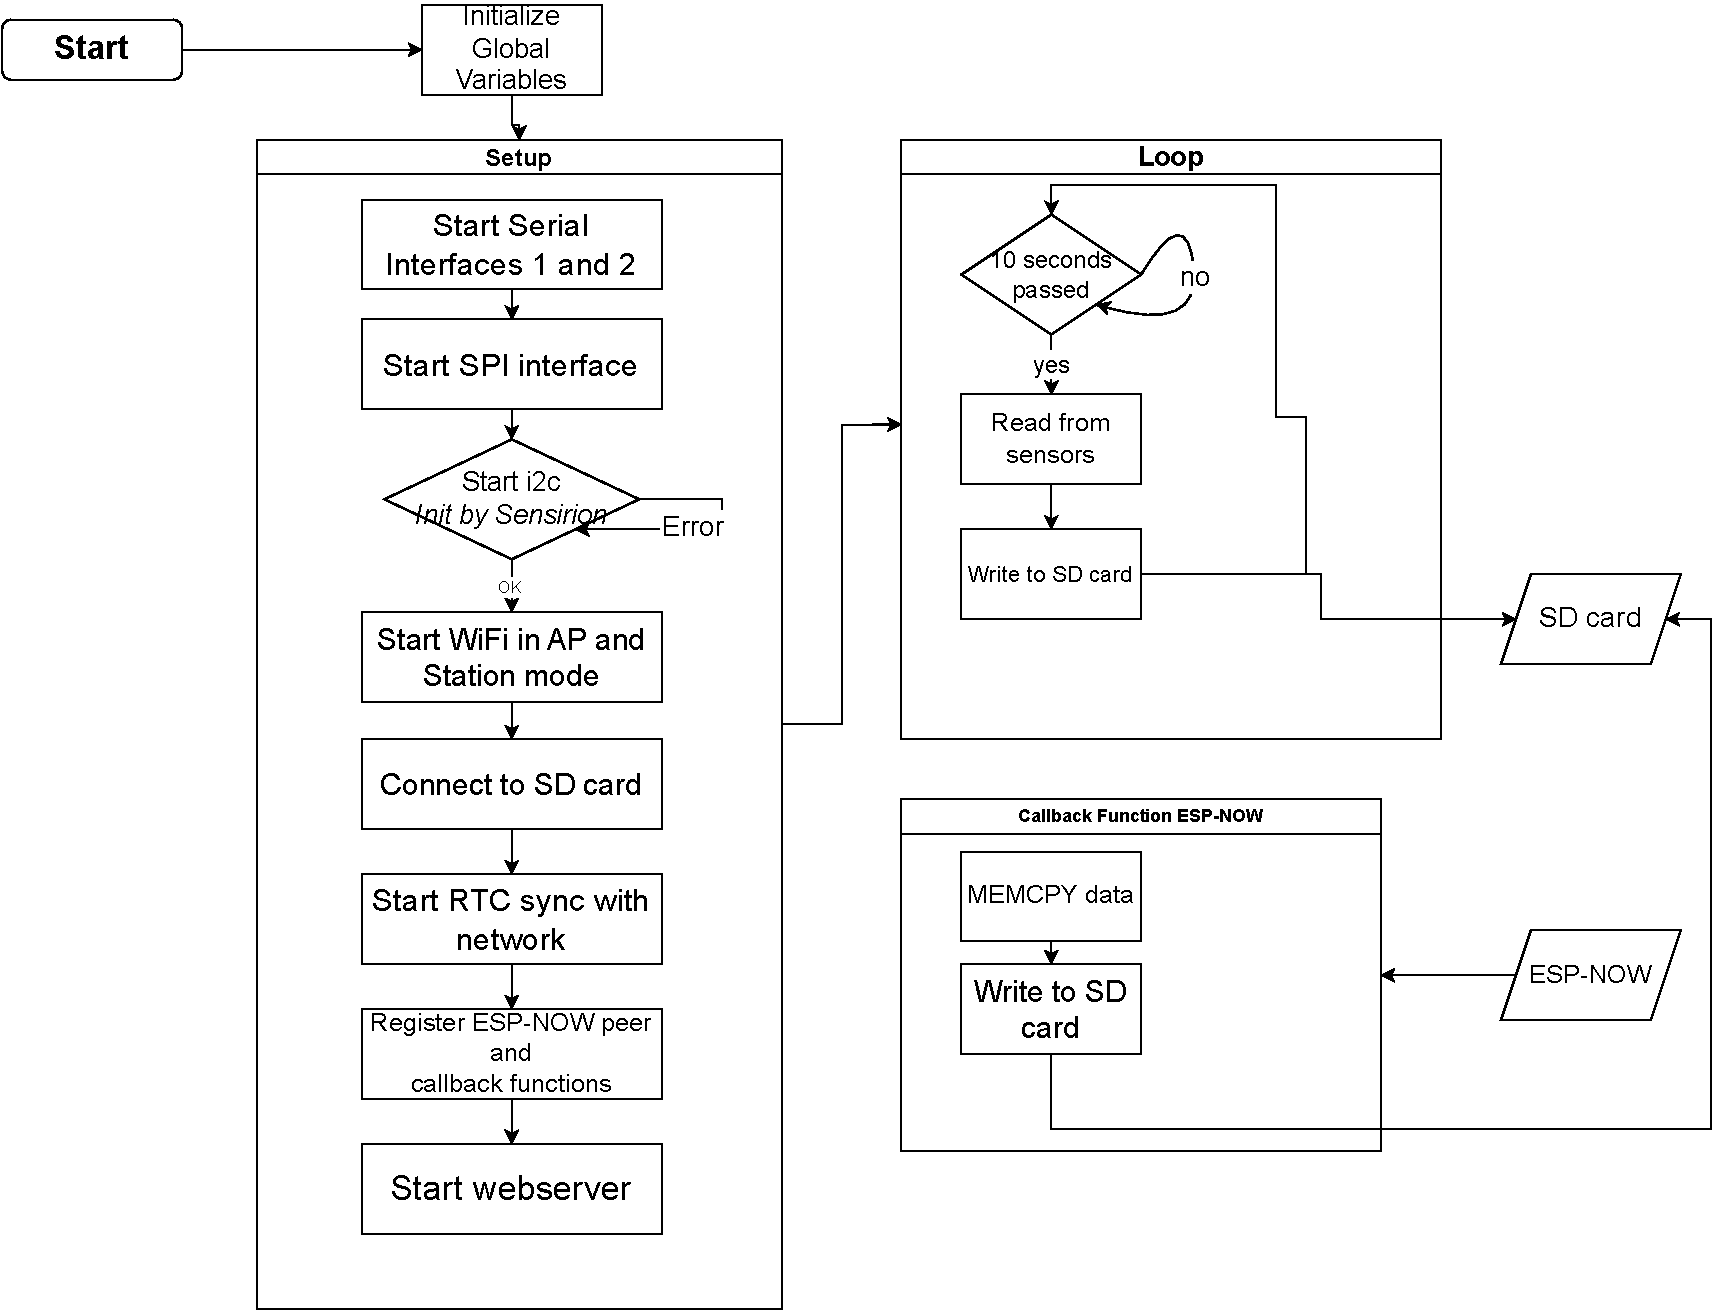
\includegraphics[width=\textwidth]{body/fig/flowchart.drawio.png}
	\caption{Flow diagram of software implementation on the base station}
	\label{fig:softwareoverview}
\end{figure}

\subsubsection{GPS and UART}
The GPS unit uses UART Serial commands to send its data to the ESP32. The data received from the GPS module is in the format of NMEA strings. This is the standard format for most GPS receivers.\cite{NMEA}
\begin{table}[!htb]
	\resizebox{\textwidth}{!}{%
		\begin{tabular}{|l|l|}
			\hline
			NMEA Sentence & Meaning \\ \hline
			GPGGA & Global positioning system fix data (time, position, fix type data) \\ \hline
			GPGLL & Geographic position, latitude, longitude \\ \hline
			GPVTG & Course and speed information relative to the ground \\ \hline
			GPRMC & Time, date, position, course and speed data \\ \hline
			GPGSA & GPS receiver operating mode, satellites used in the position solution, and DOP values. \\ \hline
			GPGSV & The number of GPS satellites in view satellite ID numbers, elevation, azimuth and SNR values. \\ \hline
			GPMSS & Signal to noise ratio, signal strength, frequency, and bit rate from a radio beacon receiver. \\ \hline
			GPTRF & Transit fix data \\ \hline
			GPSTN & Multiple data ID \\ \hline
			GPXTE & cross track error, measured \\ \hline
			GPZDA & Date and time (PPS timing message, synchronized to PPS). \\ \hline
			150 & OK to send message. \\ \hline
		\end{tabular}%
	}
	\label{tab:nmea}
	\caption{NMEA Sentences and their meanings \cite{GPSSentence}}
\end{table}

\noindent
This data is sent over the UART in comma delimited messages, the UART is set by default to 9600 baud.
The ESP32-S2 has 2 hardware UARTs, one is used for debugging and communication with the device while developing and one for communicating with the GPS module. The first UART is set to 115200 baud and the second to 9600 baud. Each UART is initialized separately and the second UART is passed to the gps encoding library TinyGPS++. The first UART is only called when debugging or notices are needed. It is used to check sending of messages using ESP-NOW for example.
The outputs from the GPS that are actually used are the date, time, longitude and latitude. This data is written to the sd card in the first header columns in the case of the satellite station.

\noindent
The data is then used to also find the distance between the satellite station and the coordinates set for the base station. The formula used to calculate the distance between the two was as follows:
\begin{equation}\label{eq:distance}
	\arccos(\sin(lat1)\times\sin(lat2)\times\cos(lat1)\times\cos(lat2)\times\cos(lon2-lon1)) \times 6371
\end{equation}
Where 6371 is the radius of the earth.

\subsection{ESP-NOW}
As mentioned in the above section, the GPS coordinates determine whether when the data from the satellite station should be sent. But before the data can be sent, a few initialization steps need to take place.
esp\_now\_init() gets called to initialize the ESP-NOW protocol, this returns ESP\_OK when done. Next the base station MAC address is written to memory and passed to the ESP-NOW handler, here the connection could be encrypted, but it is not necessary for the functionality as the data we are sending is not private. We then register the callback function that checks if the packet was sent successfully ESP\_NOW\_SEND\_SUCCESS will be returned if it was. When writing to the SD card there is a variable keeping track of the datas location, this counter serves as a means of incrementing if data has been sent before and to ensure all data was sent, if the data at receiving side is not incremental, it means we have made an error. The data sent to using the ESP-NOW protocol has a set format, it takes a struct with the format

\chapter{Results}

%First say what you are looking at. Then say what yo get from figure
%now given this what does it tell you
%for each table and figure

%{\color{red} \huge SD card not soldered \\ rest functional \\ideal implementation would be permanent\\ Will likely only encompass a days worth of data.}

\begin{figure}[!htb]
	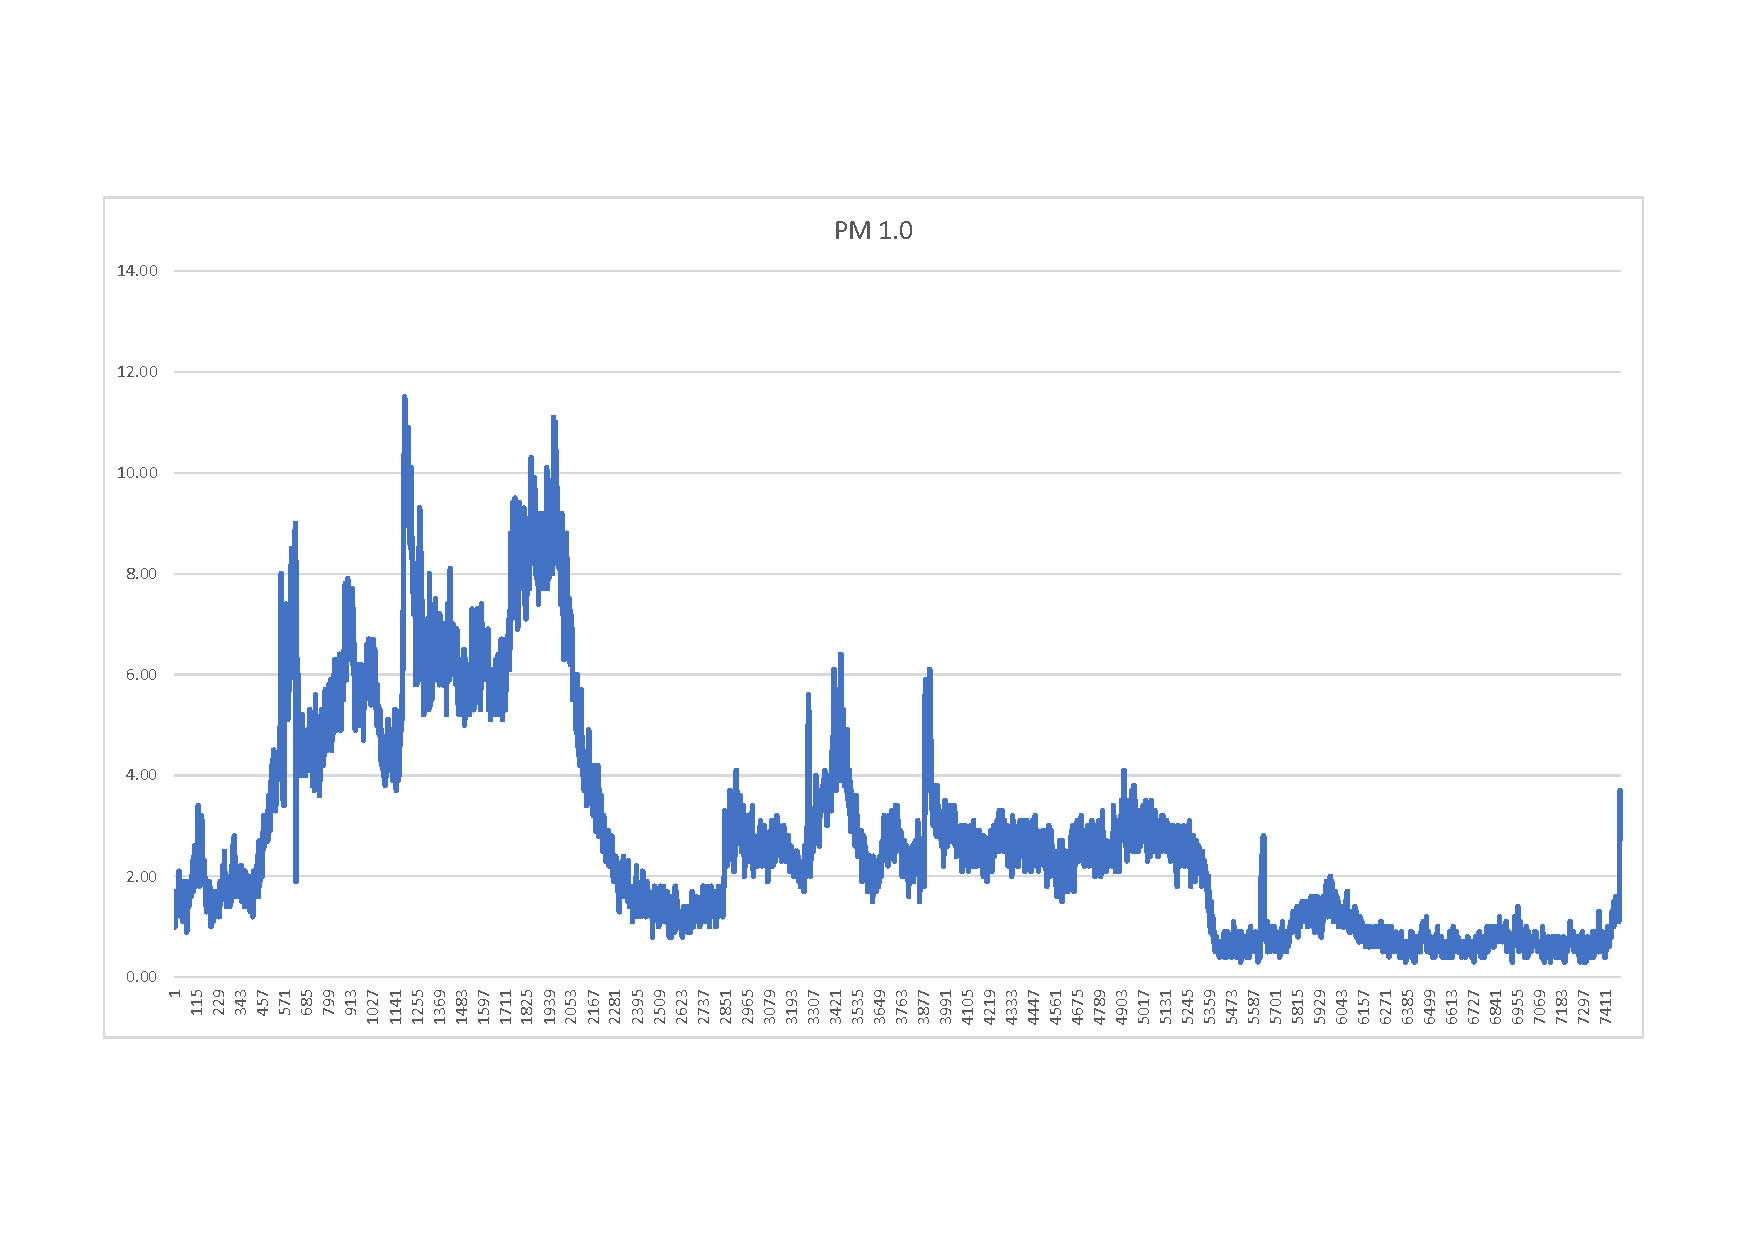
\includegraphics[width=0.45\textwidth, height = 10em]{body/fig/PM0.1.pdf}%
	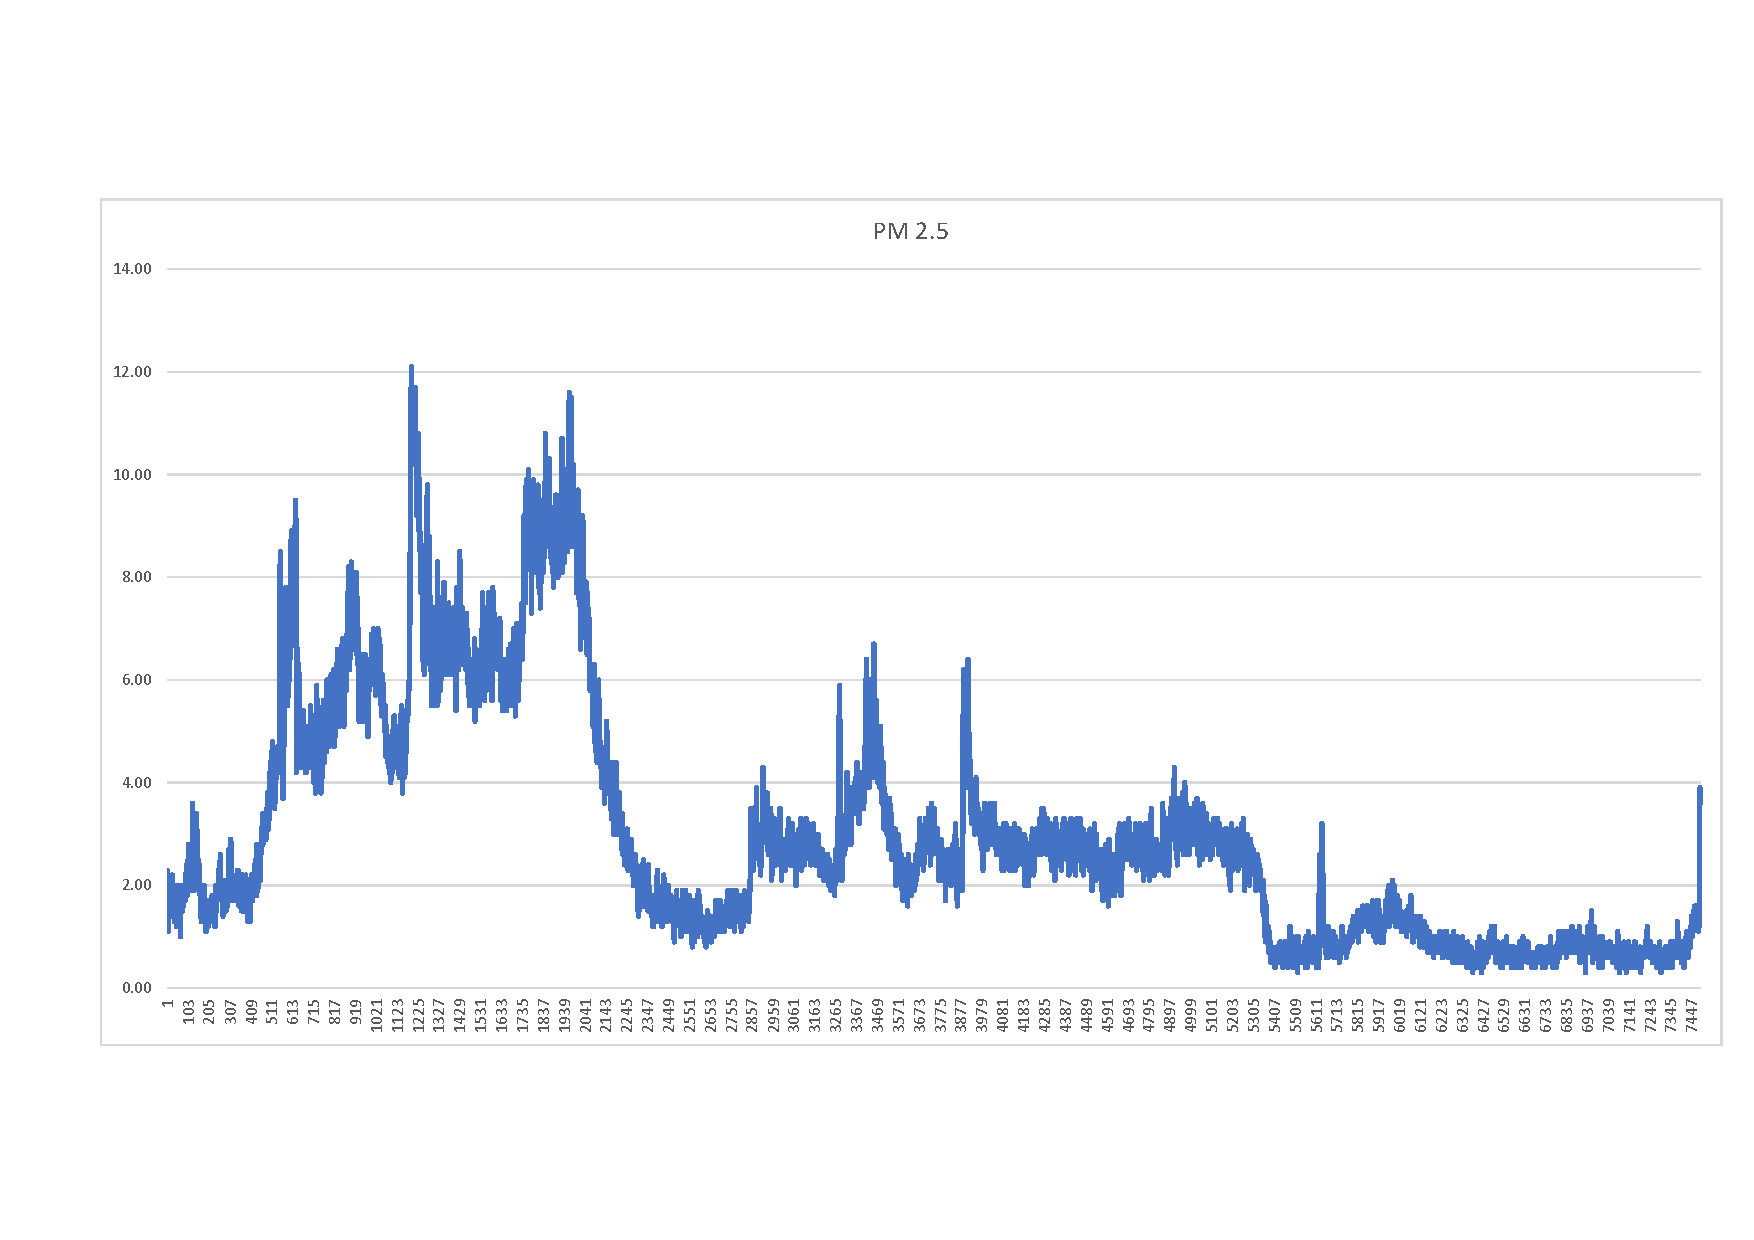
\includegraphics[width=0.45\textwidth, height = 10em]{body/fig/PM2.5.pdf}%
	\caption{PM 0.1 (left) and PM 2.5 (right)}
	\label{ACEM1}
	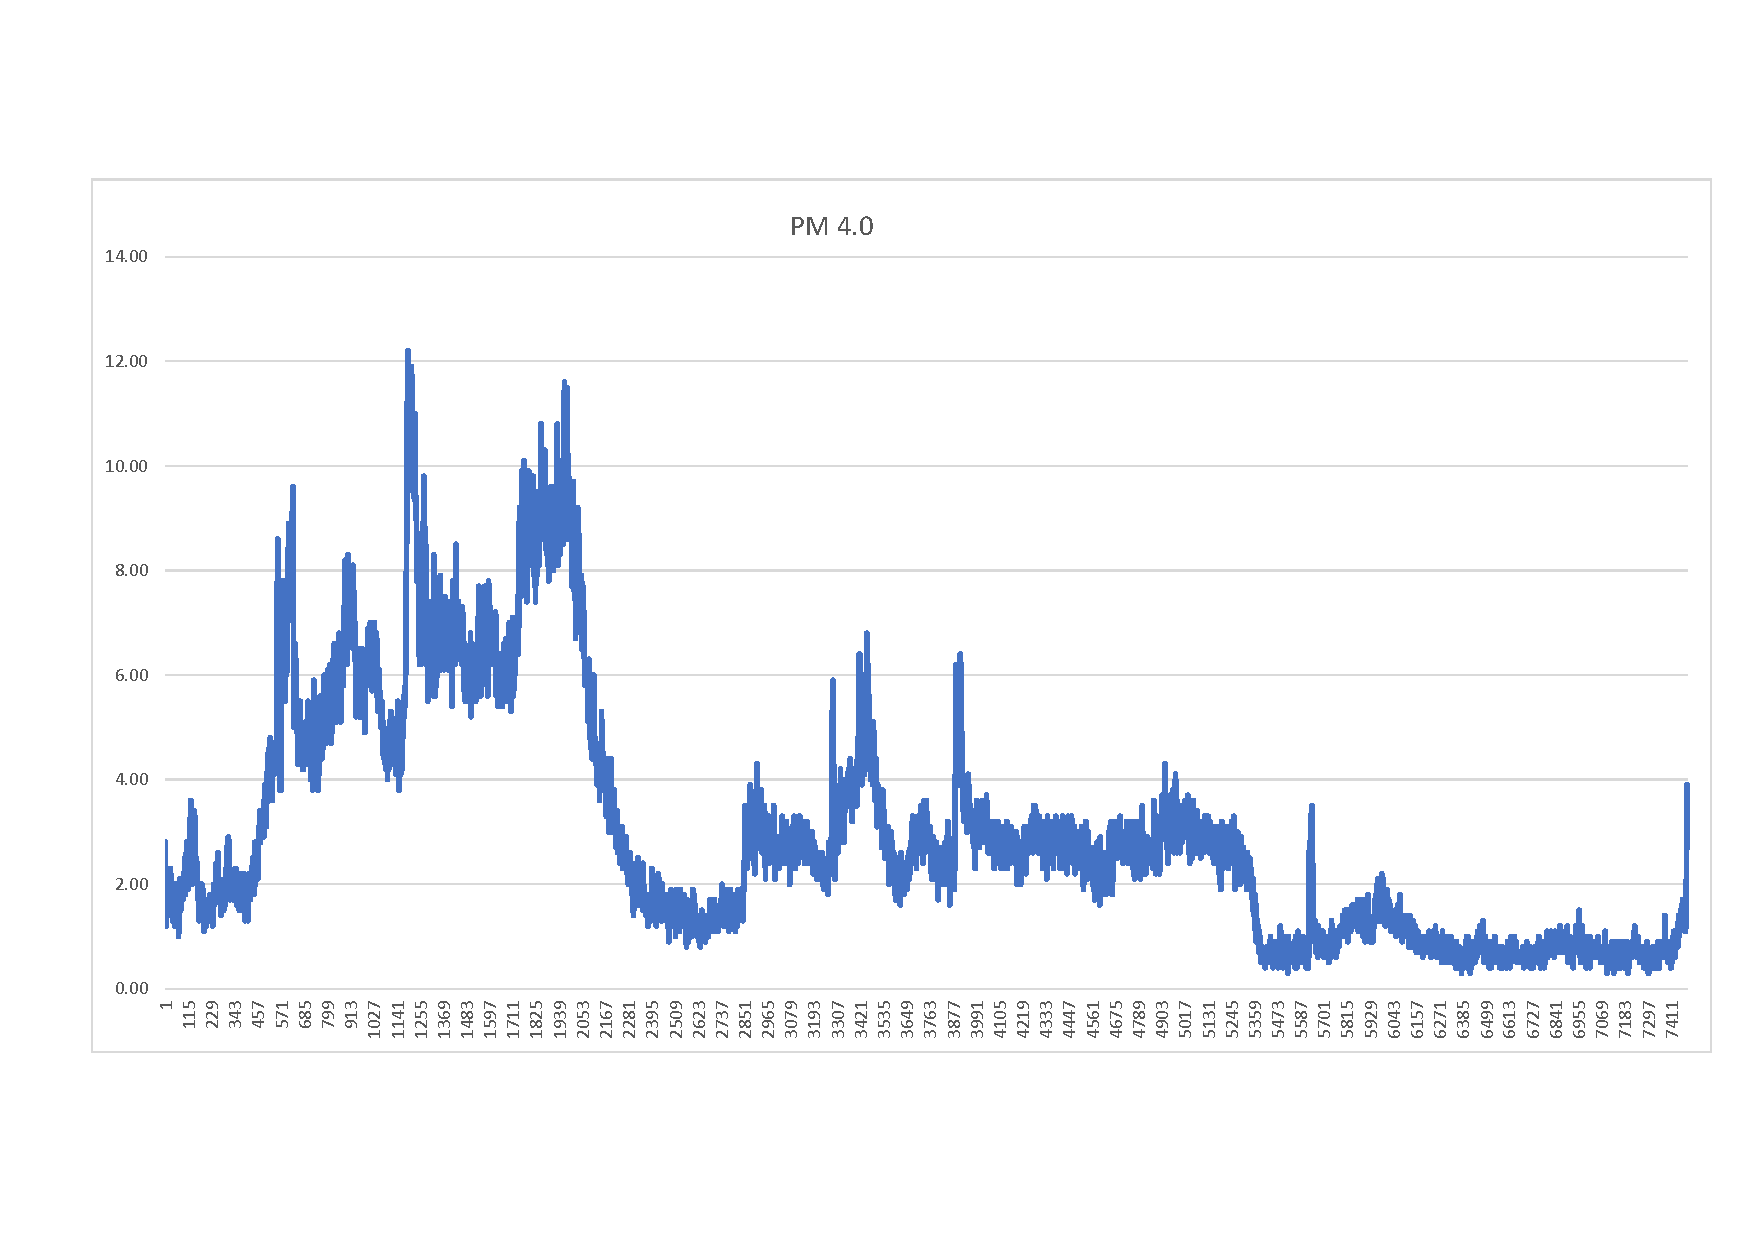
\includegraphics[width=0.45\textwidth, height = 10em]{body/fig/PM4.pdf}%
	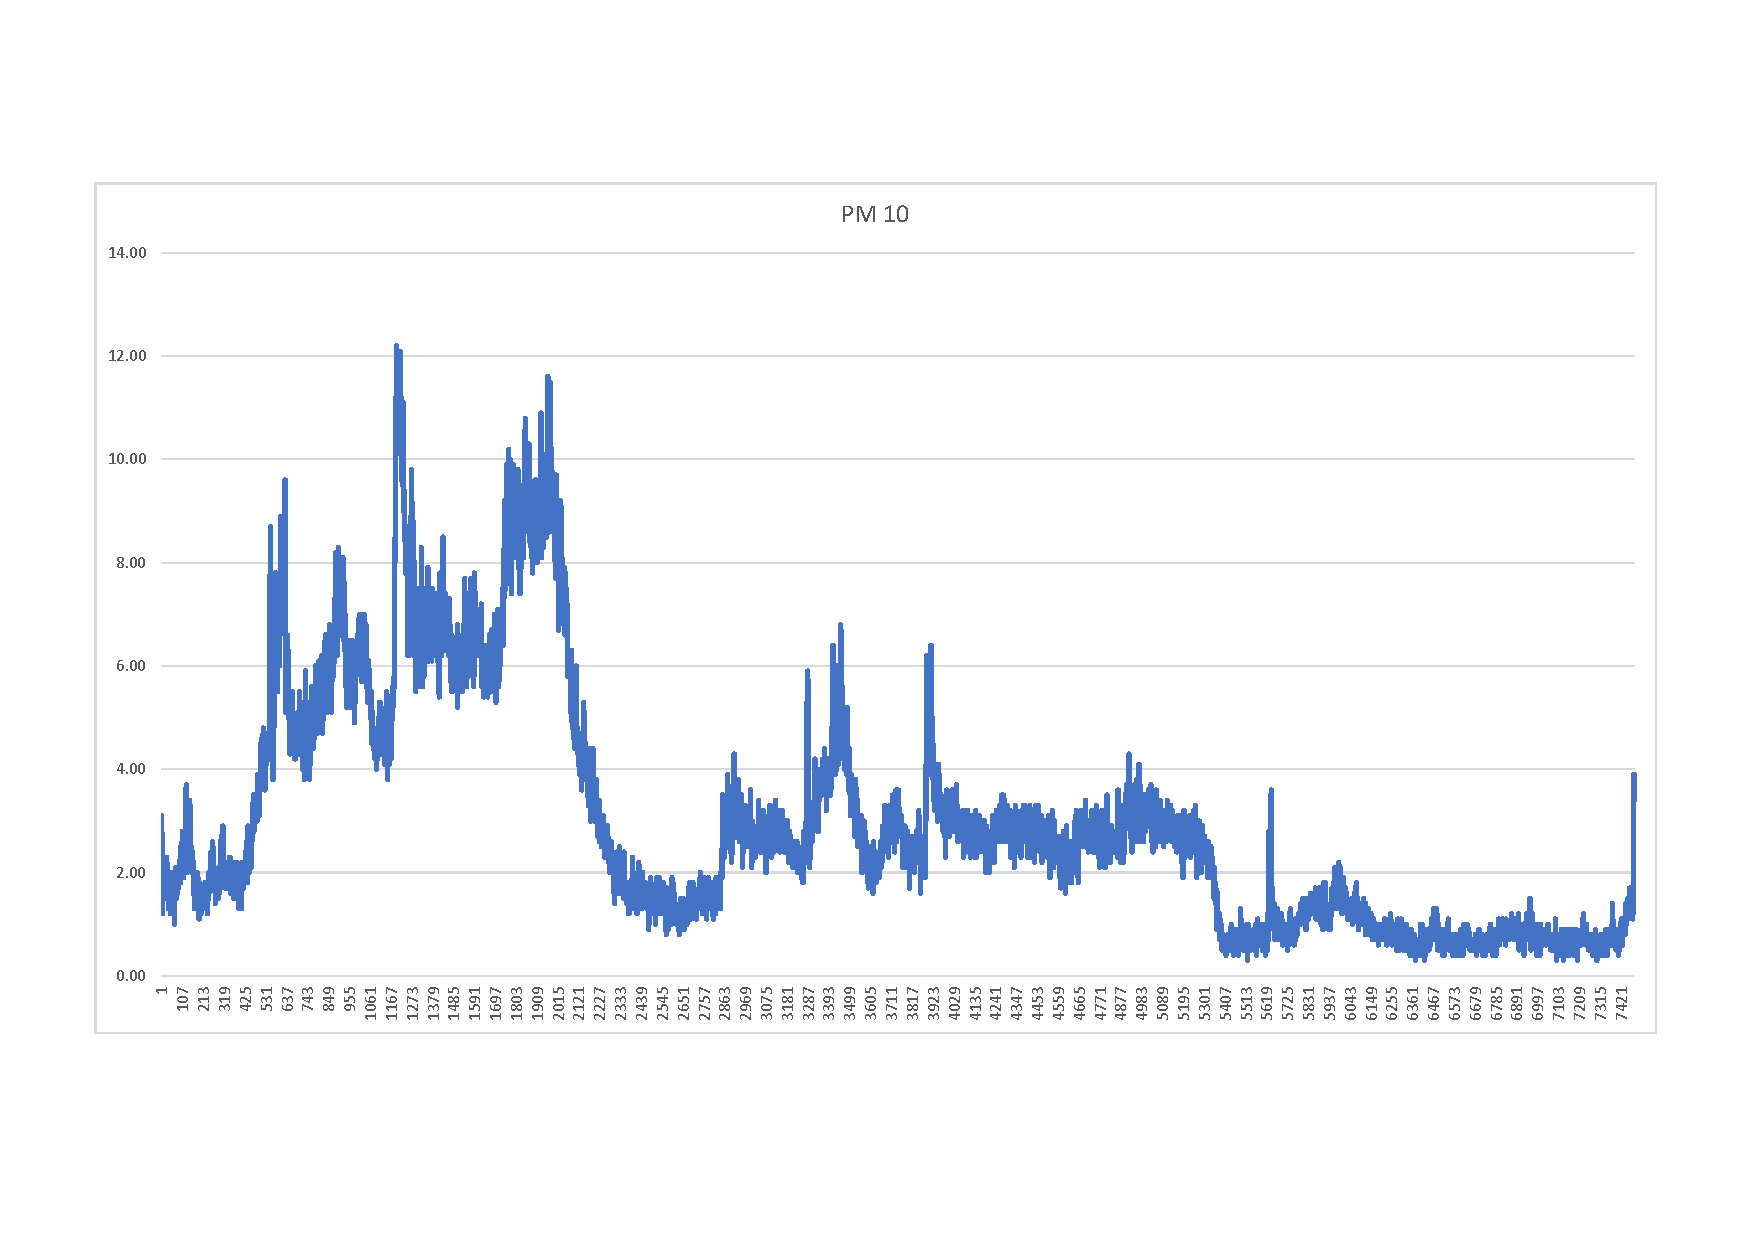
\includegraphics[width=0.45\textwidth, height = 10em]{body/fig/PM10.pdf}%
	\captionof{figure}{PM 4.0 (left) and PM 10 (right)}
	\label{ACEM2}
\end{figure}

\graphicspath{{conclusion/fig/}}

\chapter{Summary and Conclusion}
\label{chap:conclusion}
\section{Summary}

%List objectives and methods and what was gotten
The objective of this thesis was to design and build a solution to measure the air quality inside taxis and at taxi ranks. The solution built has sensors that measure CO2, particulate matter, VOC, NOx, relative humidity and temperature. The solution stores this data locally and is able to communicate between devices making it portable and easily transportable, as was the goal. The solution features connectivity and data acquisition methods, battery capabilities and 

\section{Conclusion}
%then conclusion, so what... what do you tell your granny

%future work or recommendations


% Bibliography
\bibliography{mybib}

% End matter
%\clearpage
%\pagenumbering{arabic}% resets `page` counter to 1
%\renewcommand*{\thepage}{A\arabic{page}}
\appendix
$\renewcommand\thesection{\Roman{section}}
\chapter{Project Planning Schedule}
\makeatletter\@mkboth{}{Appendix}\makeatother
\label{appen:derivations_bigramseg}

This is an appendix.

\chapter{Outcomes Compliance}
\makeatletter\@mkboth{}{Appendix}\makeatother
\label{appen:derivations_bigramseg}

This is another appendix.

\end{document}

